\documentclass{standalone}

\usepackage{xcolor}
\usepackage{graphicx}
\usepackage{tikz}

\usetikzlibrary{shapes.geometric, arrows}
\usetikzlibrary{calc,positioning}

\graphicspath{{../../}}

\begin{document}
\nopagecolor
\large
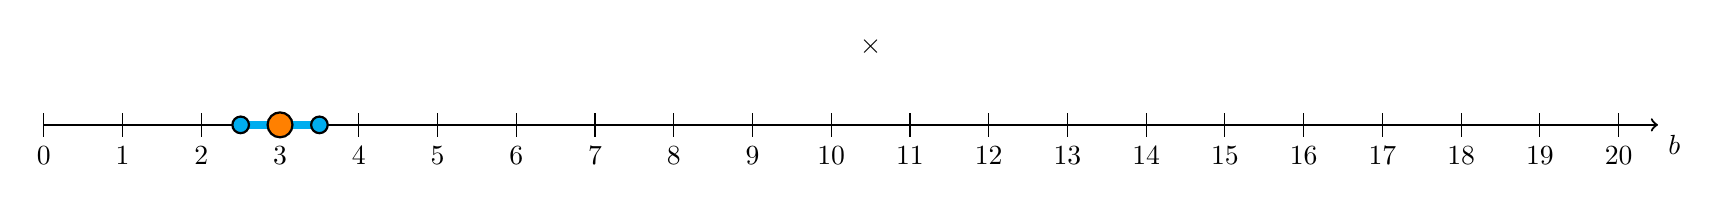
\begin{tikzpicture}[scale=1]

    \node at (10.5,1) {$\times$};

    % As
    \draw[->, thick] (0,0) -- (20.5,0)
      node[below right] {$b$}
      ;

    % Ticks
    \foreach \x in {0,...,20} {
        \draw (\x,-0.15) -- (\x,0.15);
        \node[below] at (\x,-0.15) {\x};
    }
    \draw[line width=3pt, cyan] (2.5,0) -- (3.5,0);
    \draw[fill=cyan, thick] (2.5,0) circle (3pt);
    \draw[fill=cyan, thick] (3.5,0) circle (3pt);
    \draw[fill=orange, thick] (3,0) circle (4.5pt);
\end{tikzpicture}
\end{document}
